\documentclass{article}

\usepackage{geometry}
\geometry{margin=1in}

\usepackage{graphicx}
\graphicspath{ {images/}}

\usepackage[backend=biber,style=authoryear]{biblatex}
\addbibresource{proposal.bib}

\author{Tom Wallace}

\title{Paper Proposal 
\\ \large The Rise of Slavery in America: an Agent-Based Model}

\begin{document}

\maketitle

What caused chattel slavery to emerge in the American South? This question has generated an enormous amount of
academic inquiry. Most agree that American slavery had both ideological and
economic underpinnings, but the relative importance of these two factors is
contested. The ideology camp sees slavery as driven by white supremacy: a 
``peculiar institution'' (to use John Calhoun's phrase) 
that was carried out for mostly non-economic reasons. In this view,
white Southerners believed in the inferiority of blacks and so erected an economic
system actualizing those beliefs; whether it was profitable or not was a
secondary concern. The ``new history of capitalism'' (NHC) 
emphasizes the profit-motivated nature of slavery and 
in particular its connection to the emergence of industrial capitalism
and global trade in the 19th century. In this view, white supremacist ideology was constructed as 
\textit{post hoc} intellectual justification for a money-making scheme predicated
on cheap black labor and high cotton prices. 
To simplify the debate, did racist ideology
dictate the economic system, or did the economic system dictate racist 
ideology?

Sven Beckert's \textit{Empire of Cotton}, an influential entry in the
NHC literature, offers a compelling hypothesis centered on market information,
labor mobility, and land use. The Industrial Revolution caused great demand
for foreign cotton to supply British textile mills. However, extant cotton production
in the Global South was governed more by local culture and traditions than
capitalist logic. To paraphrase, peasants in then-British India 
grew some cotton on the side because that was what they had always done, 
but they were unwilling to radically ramp up production (which would have
required abandonment of food crops and organization into large plantations rather 
than family plots) to meet the demands of Lancashire and Birmingham factories. 
There was a need for a industrial-scale cotton production system more attuned to 
global price signals. 

Beckert's hypothesis is that American slavery resulted from 
land-use and labor mobility issues associated with the creation
of such a system. Cotton is nutrient-hungry (it rapidly exhausts the soil) and labor-intensive
(land-clearing and cultivation is hard work). From the perspective of British ``cotton
capitalists'' who would eventually finance virtually all U.S. plantations, 
an ideal cotton production set-up would be highly sensitive to price signals; 
surplus land to which production could move after local soil exhaustion; 
no competition with food crops or land rights; and a highly mobile workforce 
that would follow the rapid movement of cotton farms from exhausted to
fresh soil. The early 19th century American South had almost all these
characteristics. The climate was favorable; the culture was mercantile; 
advances in communications technology (e.g. the telegraph) allowed the ever-more-rapid transmission of 
market information; the Louisiana Purchase and depopulation of Native Americans 
left a vast frontier of virgin soil. 

The only barriers were land use and labor. Free white
men had property rights and refused to totally structure their land use 
around cotton (whose price was volatile, making agricultural 
diversification a better strategy for small farmers without a large financial cushion).
They also were unwilling to pack up and move every few years to follow the path
of cotton cultivation. Slavery is argued to
have evolved as a response to these land use and labor mobility issues.
By importing Africans and stripping them of all rights, 
one could create a labor force that did not have a choice 
about how to use the land or where to move, and so could be coerced into
profit-maximizing patterns (for example, the modern geographic distribution of 
African-Americans still matches the path of cotton expansion in the
1800s, as seen in Figures 1 and 2). In essence, the NHC hypothesis is that when 
market information was local, there was little incentive
for slavery (and indeed, slavery had a surprisingly small footprint in America
in the 16-18th centuries, at least compared to its later heights); 
when markets became global, white agents independently converged on
slavery as a mechanism for  matching cotton supply in Mississippi to cotton demand in Lancashire. 

\begin{figure}[h!]
\caption{Historical distribution of cotton production}
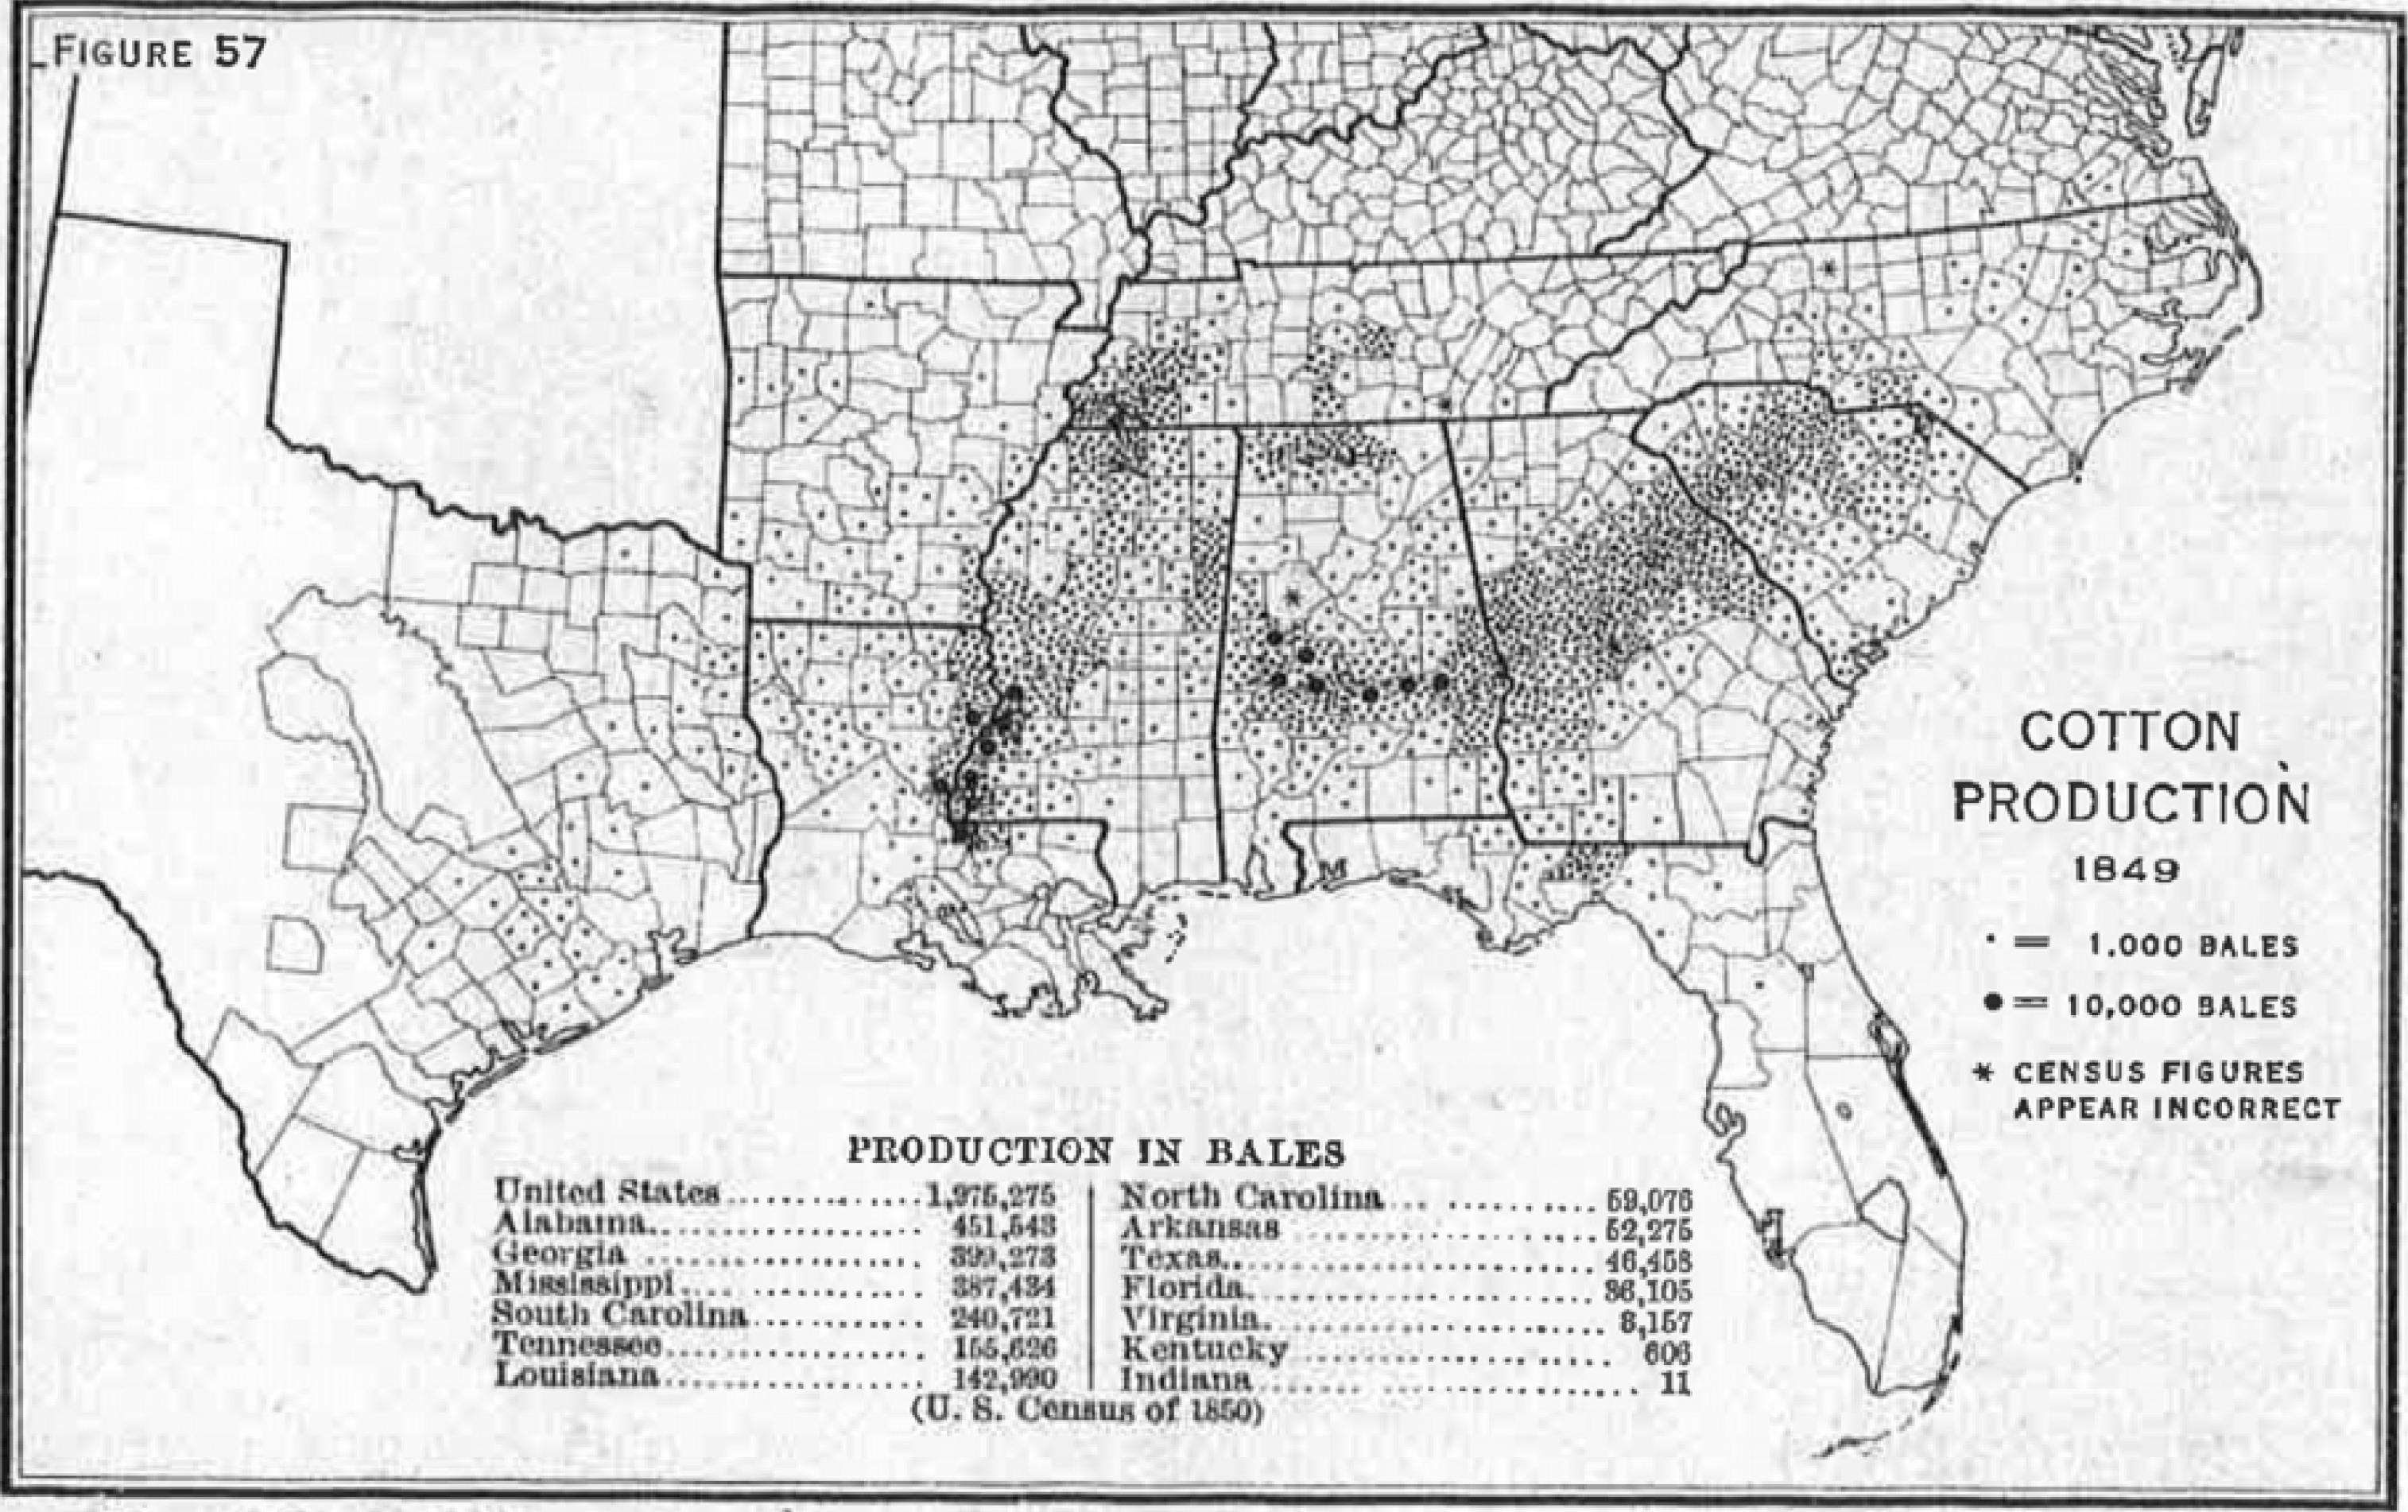
\includegraphics[scale=0.75]{historical}
\centering
\end{figure}

\begin{figure}[h!]
\caption{Current distribution of African-American population}
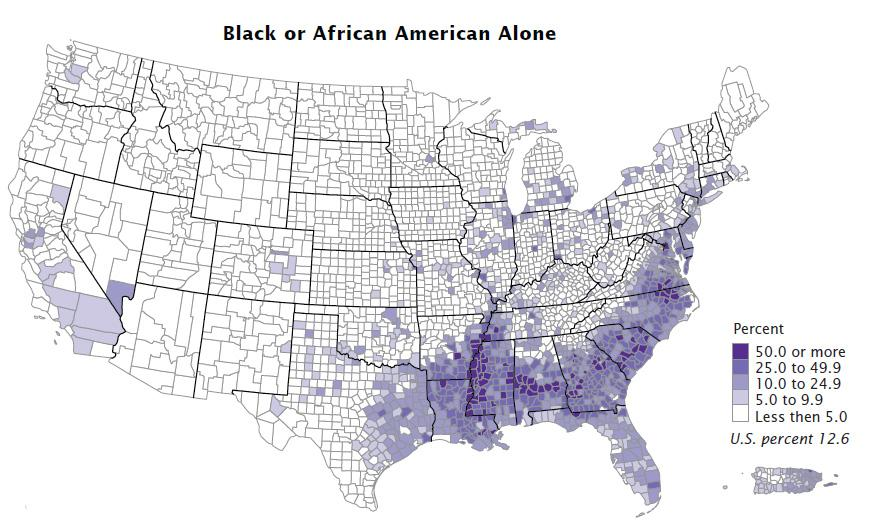
\includegraphics[scale=0.4]{current}
\centering
\end{figure}

Many aspects of the NHC hypothesis are amenable to spatial 
agent-based modeling. The NHC hypothesis relies on autonomous agents reacting to
information with boundedly rational behavior. It emphasizes the
interaction of agents with the spatial environment in terms of labor mobility
(where in the environment agents chose to go) and land-use (how they shape the
environment once there). It consists of different levels of analysis, including
both the individual and system. It emphasizes the effect of information
availability (local vs. global). These features are well-suited for agent-based
modeling.

I propose a spatial agent-based model. The environment consists of grid-square
cells. Human agents occupy these cells. Agents must decide between two land use
strategies: cotton-only or mixed cultivation. The former depletes the soil of
the grid-square while the latter can continue indefinitely. Once the soil is
depleted, the agent must move to a new grid-square. Agent cognition is governed
by preferences regarding land-use and labor mobility, and by profit motivation
based on the price of cotton and of mixed agriculture. Information regarding
prices is geographically bounded (I have not yet determined an exact mechanism
for this). The hypothesis is that increased information regarding prices causes
greater marginal value to labor mobility and land use. Clearly I have not
thought through all aspects of the model, but this is the general vision. I
likely would code this model in Python. The model would proceed in discrete
time-steps. In terms of data, I am considering obtaining GIS files of the
American South (though I do not think they are strictly necessary to explore the
hypothesis). The key dynamics that I want to model are:
\begin{itemize}
	\item Land use
	\item Labor mobility
	\item Information availability
	\item Global prices
\end{itemize}

\nocite{*}

\medskip
\printbibliography[title={}]

\end{document}

